    \documentclass[11pt,a4paper,oneside]{book}

% Include the configuration file for layout.
\usepackage{setspace}
\usepackage{geometry}
\usepackage[toc]{appendix}
\usepackage{lipsum}
\usepackage[export]{adjustbox}
\usepackage[T1]{fontenc}
\usepackage{textcomp}
\usepackage{epsfig,graphics}
\usepackage{graphicx}
\graphicspath{ {./report/assets/} }
\usepackage{titlesec}
\usepackage{amsmath,amsfonts,amssymb,amsthm}
\usepackage{hyperref}
% \usepackage{natlib}
\usepackage[printonlyused,withpage]{acronym}
\usepackage{xcolor}
\usepackage{geometry}
\usepackage{graphicx}
\usepackage{wrapfig}
\usepackage[export]{adjustbox}
\usepackage[section]{placeins}

\usepackage{algorithm}
\usepackage{algorithmic}
\renewcommand{\algorithmicrequire}{\textbf{Input:}}
\renewcommand{\algorithmicensure}{\textbf{Output:}}
\usepackage{amsmath}
\DeclareMathOperator*{\argmax}{arg\,max}
\DeclareMathOperator*{\argmin}{arg\,min}

%%%%%%%%%%%%%%%%%%%%%%%%%%%%%%%%%%%%%%%%%%%%%%%%%%%%%%%%%%%%%%%%%%%%%%%%%%%%%%
% Details of your dissertation
%%%%%%%%%%%%%%%%%%%%%%%%%%%%%%%%%%%%%%%%%%%%%%%%%%%%%%%%%%%%%%%%%%%%%%%%%%%%%%

% Fill in the following fields.
\newcommand{\projectTitle}{Planning to Explore in Reinforcement Learning}
\newcommand{\fullname}{Jared William Swift}
\newcommand{\degreeTitle}{BSc Computer Science with Artificial Intelligence (Ind)}
	% e.g. "BSc Computer Science"
\newcommand{\session}{2022/23}
	% "Session" means the academic year, i.e. 2021/22.
\newcommand{\module}{COMP3931 Individual Project}
	% e.g. "COMP3931 Individual Project".

%%%%%%%%%%%%%%%%%%%%%%%%%%%%%%%%%%%%%%%%%%%%%%%%%%%%%%%%%%%%%%%%%%%%%%%%%%%%%%
% Change the geometry of the page to have a 25 mm binding edge
%%%%%%%%%%%%%%%%%%%%%%%%%%%%%%%%%%%%%%%%%%%%%%%%%%%%%%%%%%%%%%%%%%%%%%%%%%%%%%
 \geometry{
 a4paper,
 total={210mm,297mm},
 left=25mm,
 right=25mm,
 top=25mm,
 bottom=20mm,
 }
 
%%%%%%%%%%%%%%%%%%%%%%%%%%%%%%%%%%%%%%%%%%%%%%%%%%%%%%%%%%%%%%%%%%%%%%%%%%%%%%
% Commands to set the line spacing
%%%%%%%%%%%%%%%%%%%%%%%%%%%%%%%%%%%%%%%%%%%%%%%%%%%%%%%%%%%%%%%%%%%%%%%%%%%%%%
 %\singlespacing
 \onehalfspacing
 %\doublespacing
 
%%%%%%%%%%%%%%%%%%%%%%%%%%%%%%%%%%%%%%%%%%%%%%%%%%%%%%%%%%%%%%%%%%%%%%%%%%%%%%
% Spacing for the chapter header
%%%%%%%%%%%%%%%%%%%%%%%%%%%%%%%%%%%%%%%%%%%%%%%%%%%%%%%%%%%%%%%%%%%%%%%%%%%%%%
 \titleformat{\chapter}[display]
    {\normalfont\Huge\bfseries}{\vspace*{-1\baselineskip}\chaptertitlename\ \thechapter}{15pt}{\huge}
\titlespacing*{\chapter}{0pt}{0pt}{15pt}

\renewcommand\bibname{References}

%%%%%%%%%%%%%%%%%%%%%%%%%%%%%%%%%%%%%%%%%%%%%%%%%%%%%%%%%%%%%%%%%%%%%%%%%%%%%%
% Some shortcuts that maybe useful
%%%%%%%%%%%%%%%%%%%%%%%%%%%%%%%%%%%%%%%%%%%%%%%%%%%%%%%%%%%%%%%%%%%%%%%%%%%%%%
\DeclareTextCommandDefault{\textcopyright}{\textcircled{c}}
 
%%%%%%%%%%%%%%%%%%%%%%%%%%%%%%%%%%%%%%%%%%%%%%%%%%%%%%%%%%%%%%%%%%%%%%%%%%%%%%
% Bibliography style: choose one and make sure you have the relevant .bst file
%%%%%%%%%%%%%%%%%%%%%%%%%%%%%%%%%%%%%%%%%%%%%%%%%%%%%%%%%%%%%%%%%%%%%%%%%%%%%%
\usepackage[square, numbers]{natbib}
% \setcitestyle{square}
% \bibliographystyle{numeric}
\bibliographystyle{plainnat}
% \bibliographystyle{}
%%%%%%%%%%%%%%%%%%%%%%%%%%%%%%%%%%%%%%%%%%%%%%%%%%%%%%%%%%%%%%%%%%%%%%%%%%%%%%
% Layout for the front cover !!!!! YOU SHOULD NOT HAVE TO CHANGE THIS!!!!!
%%%%%%%%%%%%%%%%%%%%%%%%%%%%%%%%%%%%%%%%%%%%%%%%%%%%%%%%%%%%%%%%%%%%%%%%%%%%%%
 
\newcommand{\frontcover}{
% The title page:
\begin{titlepage}
\newgeometry{left=25mm,right=25mm,top=45mm,bottom=0.1cm}

\begin{minipage}[t]{6cm}
\noindent\textbf{\Large{School of Computing}}\\
{\fontfamily{ptm}\selectfont 
\uppercase{faculty of engineering and physical sciences}
}
\end{minipage}
\hfill
\begin{minipage}[t]{7cm}
\vspace*{-15pt}

\includegraphics[scale=0.2,right]{logo_black.png}
\vspace*{-1pt}
\end{minipage}

\noindent\makebox[\linewidth]{\rule{\paperwidth}{0.4pt}}

\centering
\vspace*{20mm}
\textbf{\huge Final Report}\\
\vspace*{20mm}
\textbf{\Large\projectTitle}\\
\vspace*{10mm}
\textbf{\large\fullname}\\
\vspace*{10mm}
\textbf{Submitted in accordance with the requirements for the degree of}\\
\textbf{\degreeTitle}\\
\vspace*{10mm}
\session\\
\vspace*{10mm}
\module\\
\restoregeometry
\end{titlepage}
}

%%%%%%%%%%%%%%%%%%%%%%%%%%%%%%%%%%%%%%%%%%%%%%%%%%%%%%%%%%%%%%%%%%%%%%%%%%%%%%
% Define a new environment for the dissertation summary
%%%%%%%%%%%%%%%%%%%%%%%%%%%%%%%%%%%%%%%%%%%%%%%%%%%%%%%%%%%%%%%%%%%%%%%%%%%%%%
\newenvironment{dissertationsummary}
 	{\cleardoublepage \null 
 		\begin{center}%
			\textbf{Summary}
		\end{center}}%
	{\vfill \null }

\begin{document}
% The prelude is everything up to the start of chapter 1, and is contained
% in a file called "prelude.tex".
\pagenumbering{roman}
\frontcover

\clearpage

\noindent The candidate confirms that the following have been submitted.\\

% Below are examples of what your deliverables may be,
% but since every project is different, not all deliverables
% apply to all projects. Having said that, you should have
% the 'Final Report' deliverable, and most projects will also
% have a link to an online software repository.

\begin{table}[ht!]
\begin{tabular}{|p{0.3\textwidth}|p{0.3\textwidth}|p{0.3\textwidth}|}
\hline 
Items & Format & Recipient(s) and Date \\ 
\hline 
Final Report & PDF file & Uploaded to Minerva (01/05/2023) \\ 
\hline
Link to online code repository & URL & Sent to supervisor and assessor (01/05/2023) \\ 
\hline 
\end{tabular} 
\end{table}


\vfill

\noindent The candidate confirms that the work submitted is their own and the appropriate credit has been given where reference has been made to the work of others.

\vfill

\noindent I understand that failure to attribute material which is obtained from another source may be considered as plagiarism.

\vfill

% Sign this with a pen for all of the hard copies before you hand
% them over to the SSO. If for any reason the submission of final reports
% is online-only, replace the '\rule{}{}' command with your name.
\flushright(Signature of Student) JARED WILLIAM SWIFT
\flushleft

\vfill

\textcopyright~\session~The University of Leeds and~\fullname
% Summary

\begin{dissertationsummary}
Efficient exploration is imperative to success in Reinforcement Learning. However, random approaches, which are not inefficient, are often favoured in practice due to their ease of implementation and robustness. Model-based approaches to exploration are typically more sample efficient, but much of the current approaches are either very optimistic or computationally expensive, and rely on learning a model entirely from scratch and assume that it will eventually become correct.
\newline\newline Within this work we explored a model-based approach to exploration that leverages an initial model, uses a \textit{reasonable} amount of optimism, alongside intrinsic motivation, to explore and learn whilst not assuming that the model will eventually become correct. Exploration was driven by enabling the planner to hypothesise where the model may be incorrect, through additional actions denoted \textit{Meta Actions} and then realising these hypotheses through experience.
\newline\newline Various implementations were developed based on this idea, and were evaluated in a collection of gridworld-like domains, and our method of exploration was shown to perform better than the most ubiquitous random method, $\epsilon$-greedy, in most cases; moreover, the agents with \textit{Meta Actions} available to them often outperformed those without them, showing that they can be a useful exploration mechanism.
\end{dissertationsummary}

\clearpage
\centering\textbf{Acknowledgements}
\flushleft
I'd like to thank my supervisors, Dr. Mehmet Dogar and Dr. Matteo Leonetti, for their constant support and thoughts throughout this project. I'd like to thank Dr. Matteo Leonetti again, for supporting me throughout the entirity of my undergraduate degree, and for providing me with many opportunities to develop autonomous service robotics applications and take part in robotics competitions.
\\I'm grateful for the feedback from my assessor, Dr. Sebastian Ordyniak.
\\I'd like to thank my parents, for everything.


% The contents
\setcounter{tocdepth}{1}
\setcounter{secnumdepth}{4}
\tableofcontents

% The list of figures and tables. Optional.
\clearpage
%\listoffigures
%\listoftables

\pagenumbering{arabic}

 \setlength\parindent{24pt}
% Include as many chapters as you have.
% The "chapter1.tex" etc. files should be in a directory called "chapters"
% \section{List of Acronyms}
% \begin{acronym}
%  \acro{RL}{Reinforcement Learning}
%  \acro{MDP}{Markovian Decision Process}
%  \acro{POMDP}{Partially Observable Markovian Decision Process}
% \end{acronym}


\chapter{Introduction and Background Research}

% You can cite chapters by using '\ref{chapter1}', where the label must
% match that given in the 'label' command, as on the next line.
\label{chapter1}
\section{Introduction}
\begin{itemize}
    \item Reinforcement Learning (RL) is based on the concept of learning through experience - through trial-and-error.
    \item  This is akin to the way in which humans and animals learn new skills (\textcolor{red}{link to psychology}).
    \item Motivate need for exploration
    \item Exploration is a widely studied topic in RL, as it is necessary for learning. Although exploration methods exist based on optimism, \textcolor{red}{cite here}, intrinsic motivation, \textcolor{red}{cite here}, human interaction, \textcolor{red}{cite here} and information theory, \textcolor{red}{cite here}, in practice, random exploration is ubiquitous. Randomness precludes efficiency and prohibits explainability.
    \item In contrast to RL, Automated Planning uses embedded knowledge of the environment, in the form of a model, to determine the optimal sequence of successive actions required to reach a goal. However, Planning relies the model to accurately represent  the environment - this cannot be guaranteed and therefore Planning can be quite fragile.
    \item Combinations of Planning and RL have been developed in order to overcome the fragility of Planning and reduce exploration required for learning, such as DARLING \cite{AIJ16-leonetti}, where exploration is constrained to seemingly optimal states by reasoning on the model.
    \item Discuss issues with current state of the art.
    \item Within this work we explore the development of a framework that synergises planning and learning in order to drive and constrain exploration by making intelligent hypotheses about the environment, informed by the inherently inaccurate, but still useful, model, previous experience and environmental observations, rather than through randomness. The ultimate goal of this work is to mitigate the effect of the inherent inaccuracies in the model on the quality of learned behaviour; resulting in agents that can learn beyond the inaccuracies of the model, through intelligent exploration.
\end{itemize}
Reinforcement Learning (RL) is based on the concept of learning through experience - it is a form of trial-and-error learning. An agent learns how to behave in an environment by interacting with it and receiving reinforcement (both positive and negative) through a numerical signal called the reward.
RL is grounded in psychology 

This is akin to the way in which humans and animals learn new skills 
\section{Reinforcement Learning}
Reinforcement Learning (RL) does not fall into either of the traditional machine learning paradigms (supervised and unsupervised learning) - it is a machine learning paradigm of its own. Within an RL problem a goal-directed decision-making agent learns how to behave in an environment (which may be stochastic). The agent learns by interacting with the environment through actions and observing the affects through its new state and a numerical reward signal. The goal of the agent is to learn how to map states to actions in order to maximise the cumulative long-term reward signal \cite{DBLP:books/lib/SuttonB98}.
A Model-Free RL agent has 3 elements:
\begin{itemize}
    \item \textbf{Policy}
    \item \textbf{Reward}
    \item \textbf{Value}
\end{itemize}
A Model-Based RL agent has the same elements as that in the Model-Free setting, but additionally it has a Model. The model may be learnt by the agent in order to plan on, or it may be given to the agent to inform exploration.
Within the Introduction we motivated the need for exploration, however we did not mention a key problem in RL; the \textit{exploration-exploitation trade-off}. The agent needs to explore in order to gain experience and learn, but it must also exploit its learned knowledge - the problem is knowing when to explore and when to exploit.
\subsection{Markov Decision Processes}
The Markov Property states that the future is conditionally independent of the past given the present. An RL problem that satisfies the Markov Property is known as a Markov Decision Problem, and can be modelled by a Markov Decision Process (MDP). MDPs can be fully (MDP) or partially observable (POMDP). Consider an agent interacting with a stochastic gridworld, the agent can easily observe its state, whereas a robot navigating a maze may not be able to observe its exact state, due to uncertainty in sensors, joint readings, etc. In fact, the real-world is a POMDP. Within this work, as a simplification, we assume that the agent is fully able to observe its state. Furthermore that the environment can be discretised (rather than being modelled in a continuous nature); hence we consider \textbf{finite} MDPs.
A finite MDP is a 4-tuple: $\text{MDP} = (S,A,T,R)$ where:
\begin{itemize}
    \item $S$ is a finite set of states.
    \item $A$ is a finite set of actions.
    \item $T : S \times A \times S \rightarrow [0,1]$ is the transition function, which determines the probability of transitioning from a state $s \in S$ to $s' \in S$ with an action $a \in A$.
    \item $R:S \times A \times S \rightarrow \mathbb{R}$ is the reward function, which determines the reward signal, $r \in \mathbb{R}$ received by the agent from transitioning from a state $s \in S$ $s' \in S$ with the action $a \in A$. This reward is extrinsic to the agent; it comes from the environment.
\end{itemize}
The transition function, $T$ is a key indicator about the nature of the environment.
If $\forall s,s' \in S, \forall a \in A$, $T(s,a,'s) \in \{0,1\}$, then the environment is deterministic, otherwise it is probabilistic.
A deterministic environment is one which there is no variance in the outcomes of action in a given state; taking the same action in the same state always produces the same outcome. Whereas a probabilistic (or non-deterministic) environment has uncertainty associated with transitions.
\\The Bellman Equation determines the expected reward for being in a state $s \in S$ and following a fixed policy $\pi$:
$$V^\pi(s) = R(s, \pi(s)) + \gamma \sum_{s'}P(s'|s,\pi(s))V^\pi(s')$$
Where $V^\pi$ is the value function of the policy, $\pi$, $0 \le \gamma \le 1$ is the discount factor.
The Bellman Optimality equation determines the reward for taking the action giving the highest expected return.
$$V^{\pi*}(s) = \text{argmax}_a{R(s,a) + \gamma\sum_{s'}P(s'|s,a)V^{\pi*}(s')}$$
Where $V^{\pi*}$ is the value function of the optimal policy, $\pi*$, $0 \le \gamma \le 1$ is the discount factor.
\subsection{Model-Free RL}
\subsection{Model-Based RL}
\subsection{Dynamic Programming}
\begin{itemize}
\item Given a perfect model of the environment, embedded in a MDP, an optimal policy can be computed using Dynamic Programming. However, this assumption of a perfect model is flawed.
\end{itemize}
\subsubsection{Policy Iteration}
\subsubsection{Value Iteration}
\subsection{Temporal Difference Learning}
\begin{itemize}
    \item The (temporal) credit assignment problem.
    \item Temporal Difference (TD) learning is driven by the error/difference between temporally successive predictions; learning occurs whenever there is a change in prediction over time. \cite{Sutton:1988}
    \item Temporal difference methods bootstrap from previous experience.
\end{itemize}
\subsubsection{Q-Learning: Off-Policy TD-Learning}
\begin{itemize}
    \item Q-Learning is an off-policy Temporal Difference Learning method. It is also model-free. \cite{Watkins:1989, journals/ml/WatkinsD92}.
    \item Off-policy refers to the fact that the value of the optimal policy is learnt independently of the agent's actions, as opposed to on-policy learning where the value of the policy being carried out by the agent is learnt \cite{PooleMackworth17}.
\end{itemize}
\subsubsection{SARSA: On-Policy TD-Learning}
    \item SARSA is an on-policy TD-Learning method.
\section{Planning}
\begin{itemize}
    \item Planning involves reasoning on a model of an environment in order to produce a sequence of actions that will achieve a goal.\cite{russelNorvig2003:aima}.
\end{itemize}
\subsection{A* Search}
\begin{itemize}
    \item A* Search \cite{4082128} is not necessarily a Planning algorithm, rather it is a search algorithm. However, a simple Planning agent with the purpose of navigation in a discretised state space can use A* for planning.
    \item Heuristic
    \item Admissable
\end{itemize}
\section{Exploration in Reinforcement Learning}
\begin{itemize}
    \item \cite{Thrun-1992-15850} distinguished exploration methods into two categories: directed and undirected. A more recent work \cite{DBLP:journals/corr/abs-2109-00157} distinguished between reward-free and reward-based exploration.
\end{itemize}
\subsection{Random}
\subsection{Optimism}
\subsection{Intrinsically Motivated}
\subsection{Deliberate}

% \begin{itemize}
%     \item $\epsilon$-greedy 
%     \item 

% \subsection{Directed}
% \subsubsection{Intrinsically Motivated}
% \subsubsection{Optimistic}
% \subsubsection{Deliberate}
% \subsection{Undirected}
% \subsubsection{Blind Exploration}
\section{Related Work (Planning and Learning)}
\begin{itemize}
    \item DARLING
    \item Dyna
    \item AlphaGo?
\end{itemize}
\chapter{Background Research \& Notation}
\label{chapter2}
\section{Markov Decision Processes}
The Markov Property states that the future is conditionally independent of the past given the present. A sequential decision-making problem that satisfies the Markov Property is known as a Markov Decision Problem, and can be modelled by a Markov Decision Process (MDP) \cite{10.5555/528623}. Where an agent is able to fully observe its state, the problem can be modelled as an MDP. Conversely, where an agent can only partially observe its state, the problem can be modelled by a Partially Observable Markov Decision Process (POMDP).
Consider an agent playing a perfect information game \cite{vonneumann.morgenstern47}, such as Chess or Go, the agent (and it's opponent) are able to fully observe the state of the game with ease. Conversely, a robot navigating through a maze may not be able to observe its exact state due to uncertainty (which is guaranteed) in its sensors.
\\Within this work we assume that the agent is fully able to observe its state. Furthermore that the environment can be discretised (due to some approximations) and tasks are episodic (there exist some terminal states which indicate the end of a task); hence we consider \textbf{finite}, \textbf{undiscounted} MDPs.
Thus, an MDP is a 4-tuple: $\text{MDP} = (S,A,T,R)$ where:
\begin{itemize}
    \item $S$ is a finite set of states.
    \item $A$ is a finite set of actions.
    \item $T : S \times A \times S \rightarrow [0,1]$ is the transition function, which determines the probability of transitioning from a state $s \in S$ to $s' \in S$ with an action $a \in A$.
    \item $R:S \times A \times S \rightarrow \mathbb{R}$ is the reward function, which determines the reward signal, $r \in \mathbb{R}$ received by the agent from transitioning from a state $s \in S$ to $s' \in S$ with the action $a \in A$. This reward is extrinsic to the agent; it comes from the environment.
\end{itemize}
The transition function, $T$ is a key indicator about the nature of the environment.
If $\forall s,s' \in S, \forall a \in A$, $T(s,a,'s) \in \{0,1\}$, then the environment is deterministic, otherwise it is stochastic.
A deterministic environment is one which there is no variance in the outcomes of action in a given state; taking the same action in the same state always produces the same outcome. Whereas a stochastic (or non-deterministic) environment has uncertainty associated with transitions.
\subsection{Policies}
\subsection{Value Functions}
\subsection{Bellman Equations}
The Bellman Equation determines the expected reward for being in a state $s \in S$ and following a fixed policy $\pi$:
$$V^\pi(s) = R(s, \pi(s)) + \sum_{s'}P(s'|s,\pi(s))V^\pi(s')$$
Where $V^\pi$ is the value function of the policy, $\pi$.\\
The Bellman Optimality equation determines the reward for taking the action giving the highest expected return.
$$V^{\pi*}(s) = \text{argmax}_a{R(s,a) + \sum_{s'}P(s'|s,a)V^{\pi*}(s')}$$
Where $V^{\pi*}$ is the value function of the optimal policy.

\section{Planning and Searching}
Planning involves reasoning on a model of an environment in order to produce a sequence of actions that will achieve a specified goal \cite{DBLP:books/aw/RN2020, Lav06, GhallabNauTraverso04}.
\subsection{Heuristic Search}
Heuristic search uses heuristic functions to guide the exploration of possible solutions.
\subsubsection{A* Search}
A* search is a heuristic search algorithm, which is limited to discrete state and action spaces. It can be difficult to choose the heuristic, the heuristic must be admissable \cite{DBLP:books/aw/RN2020}; this means that it must always underestimate the cost of getting from the current state to the goal, and never overestimate it. An interesting extension of this is LRTA* \cite{KORF1990189}, which is akin to model-based RL. In the context of gridworlds, the chosen heuristic in this work is the Manhattan Distance \cite{krause1973taxicab}.
\subsection{Dynamic Programming}
Dynamic Programming \cite{Bellman:1957, DBLP:books/lib/Bertsekas05} is a problem-solving method which involves breaking down problems into smaller sub-problems, solving them, storing the solutions, and combining them to solve the original problem. Given a perfect model of the environment, embedded in an MDP, an optimal policy can be computed using Dynamic Programming, through both Policy Iteration  and Value Iteration.
\subsection{Policy Improvement}
Policy Improvement \cite{Bellman:1957} is the process of generating a policy from a suboptimal policy \cite{DBLP:books/lib/Bertsekas05}.
\subsection{Policy Iteration}
\cite{Bellman:1957, howard:dp}
\subsection{Value Iteration}
\cite{series/synthesis/2010Szepesvari}
\section{Reinforcement Learning}
Reinforcement Learning (RL) does not fall into either of the traditional machine learning paradigms (supervised and unsupervised learning); it is a machine learning paradigm of its own \cite{DBLP:journals/corr/cs-AI-9605103}.
A RL problem comes in the form of a sequential-decision making problem within an environment. A sequential-decision making problem is a problem within which the consequences of actions may not be known until long after they are taken \cite{barto1990learning}. The decision-making agent learns how to behave in an environment by interacting with the environment, at discrete time steps, through actions and observing the affects through its new state and a scalar reward signal, which may be delayed. The goal of the agent is to learn how to map states to actions in order to maximise the cumulative long-term reward \cite{Sutton1998}. The behaviour that the agent learns is called the \textbf{policy}, which is the mapping from states to actions. The \textbf{value function} indicates the expected cumulative reward the agent can receive starting from a given state, given the current knowledge of the agent obtained through its experiences thus far.

\subsection{Model-Free versus Model-Based RL}
Model-Free (or direct) RL is the traditional instantiation of RL, where an agents learns to act in an environment with no knowledge, or consideration, of its dynamics.
Model-based (or indirect) RL is where an agent uses a known or learned model (in the form of an MDP) to learn a policy \cite{MAL-086, RLSOTA11}. The learned model may be approximate or exact. The agent may learn the model and policy at the same time, as in the Dyna family \cite{Sutton:1990, 10.1145/122344.122377} or learn a policy by planning over a known model, as in AlphaZero \cite{DBLP:journals/corr/abs-1712-01815} or planning over a learned model, as in MuZero \cite{DBLP:journals/corr/abs-1911-08265}.

% The agent learns to act in the environment by either learning or being provided with a representation of the dynamics of the environment.
% Model-based RL is where the agent learns to act in an environment, and has some understanding of the dynamics of the environment in the form of a model. By the nature of models, the model is inaccurate, more often than not. \cite{Sutton:1990, MAL-086, 10.1145/122344.122377, Kuvayev1996ModelBasedRL, RLSOTA11}
\subsection{Temporal Difference Learning}
The (temporal) credit assignment problem \cite{Minsky:1961:ire} is the problem of determining which actions led to an outcome, and assigning credit among them; it's often the case that a sequence of actions led to an outcome, rather than a single action. In the context of RL, temporal credit assignment is important because in order to maximise the cumulative long-term reward, the agent needs to know which actions will realise such outcome. Temporal Difference (TD) \cite{10.5555/911176, 5392560, 5391906} learning uses this concept; learning is driven by the error/difference between temporally successive predictions, so learning occurs whenever there is a change in prediction over time. It's a method for learning to predict; learning a prediction from another later learned prediction.
TD Learning algorithms can be on-policy, such as SARSA \cite{rummery:cuedtr94}, where the value of the policy being currently carried out by the agent is learnt, or off-policy, such as Q-Learning \cite{Watkins:1989, journals/ml/WatkinsD92}, where the value of the optimal policy is learnt independently of the agent's actions following the current policy \cite{PooleMackworth17}.
\subsubsection{Q-Learning}
Q-Learning is an off-policy Temporal Difference Learning method. It learns an estimate of the expected cumulative reward for each state-action pair, this is known a the Q-value. Q-values are iteratively updated using the Bellman equation, the update rule is as follows:
$$Q(s_t,A_t) \leftarrow Q(s_t,a_t) + \alpha[r_{t+1} + \max_aQ(s_{t+1}, a) -Q(s_t,a_t)]$$
Where $0 \le \alpha \le 1$ is the learning rate, which indicates how quickly learning occurs.
\\Clearly Q-Learning comes from Dynamic Programming, and in that sense it is a tabular method; a Q-table is maintained which stores the Q-values for each state-action pair. For this reason, it doesn't scale too well to large state/action spaces - however it is suitable for the domains that we consider within this work.
\\The result of Q-Learning is that a deterministic, greedy policy is learned.

\section{Exploration in Reinforcement Learning}
Thrun \cite{Thrun-1992-15850} distinguished exploration methods in to two main categories: directed and undirected. Directed exploration refers to exploration that is informed by memory about the state space, whereas undirected exploration is uninformed, random. Due to the advances in exploration methods, these categories became redundant, and Amin et al's \cite{DBLP:journals/corr/abs-2109-00157} comprehensive survey on exploration in RL distinguished between reward-free and reward-based exploration; each of these categories is then broken down into memory-free (undirected) and memory-based (directed) exploration. We consider this taxonomy of exploration methods.
\subsection{Random Exploration}
Due to simplicity of implementation and ease of generalisation, random exploration is the most popular form of exploration, and is widely seen in the literature; even where some other exploration method is used, there is often some underlying randomness.
\subsubsection{Random Walk}
A Random Walk, or unguided random search \cite{anderson86}, arises from randomly sampling actions with uniform probability. This is perhaps the most naive method of exploration, since it is entirely random. The agent only explores and doesn't exploit; unless it learns a value function whilst exploring which it switches to exploit after some number of discrete time steps.
\subsubsection{$\epsilon$-greedy}
$\epsilon$-greedy \cite{Watkins:1989, conf/nips/Sutton95} uses a hyperparameter, $0 \le \epsilon \le 1$ to balance between exploration and exploitation. With probability $\epsilon$ the agent explores by taking a random action, with probability $1-\epsilon$ the agent exploits by taking the current best action. A key drawback of $\epsilon$-greedy exploration is that is lacks temporal persistence. Furthermore, by the nature of the name, it is a greedy method which could lead to a local optima.
\subsubsection{$\epsilon z$-greedy}
$\epsilon z$-greedy \cite{dabney2021temporallyextended} is an extension to $\epsilon$-greedy that uses temporal persistence; the agent follows a sequence of actions (an option \cite{SUTTON1999181}) until termination with probability $\epsilon$ and with probability $1-\epsilon$ the agent exploits by taking the current best action.
% \begin{itemize}
%     \item Pure random exploration: Random Walk
%     \item $\epsilon$-greedy \cite{Watkins:1989, conf/nips/Sutton95}
%     \item $\epsilon z$-geedy \cite{dabney2021temporallyextended, SUTTON1999181}
%     \item Softmax
%     \item Boltzmann \cite{Watkins:1989, 10.1007/BF00992699, SCC.Barto.Bradtke.ea1991}
% \end{itemize}
\subsection{Intrinsically Motivated Exploration}
\cite{scott1996, pmlr-v97-jinnai19b, Jinnai2020Exploration}
\subsection{Optimistic}
\cite{10.1145/1390156.1390288, NIPS2006_c1b70d96, 10.1162/153244303765208377, NIPS2008_d5cfead9}
\subsection{Model-Based}
We refer to Model-Based exploration as any method of exploration that uses a model to influence exploration. For instance, a simple form of model-based RL where an agent plans on an initial model, and performs model-learning concurrently is an exploration method; although a naive one, that doesn't work in practice.\\
\cite{SARA07-jong, Littman2011EfficientME, Epshteyn2008ActiveRL}
\subsubsection{DARLING}
DARLING \cite{AIJ16-leonetti} computes a partial policy from an approximated deterministic model which it then performs $\epsilon$-greedy on. This leads to constraining exploration to a set of seemingly reasonable states, enabling the agent to overcome inaccuracies in the model, although the model is not explicitly learned. The main problem in this approach, is that it is only suitable for where the inaccuracies are not too significant, so there is a reliance on the embedded model being somewhat correct. Furthermore, randomness is present still.
\subsubsection{PEORL}
PEORL \cite{DBLP:journals/corr/abs-1804-07779}
\subsubsection{Plan-Q Learning}
\cite{10.1007/978-3-540-77949-0_6}
\subsubsection{FRAP}
\cite{DBLP:journals/corr/abs-2006-15009}
\subsubsection{Guided Dyna-Q}
\cite{Hayamizu2021GuidingRE}
\subsection{TMP}
\cite{Jiang2019TaskMotionPW}

% Randomnes underlies most exploration strategies in RL, from using pure-randomness, to randomly samplin
% \subsection{Random}
% \subsubsection{$\epsilon$-greedy}
% $\epsilon$-greedy \cite{Watkins:1989, conf/nips/Sutton95} aims to balance exploration and exploitation through an $\epsilon$ factor, such that the agent exploits its learned knowledge, taking the current best action, with probability $1-\epsilon$ and explores randomly with probability $\epsilon$. It's common to decay $\epsilon$ temporally, so that the agent explores a lot early on and then exploits more after it has learnt for a while. Whilst this method offers a nice balance between the two extremes of pure exploration and pure exploitation, it only provably converges to an optimal policy with an infinite number of observations, so in-fact it is quite inefficient. Furthermore, due to the random nature, it results in continually evaluating sub-optimal actions. A key drawback to $\epsilon$-greedy is that without infinite observations, it can easily get stuck in a local optima.
% \subsubsection{$\epsilon z$-greedy}
% Dabney, et al., \cite{dabney2021temporallyextended} stated that another key problem with $\epsilon$-greedy is its lack of temporal persistence; actions are only performed for one time-step. They proposed $\epsilon z$-greedy, or temporally extended $\epsilon$-greedy, where the agent takes the current best action with probability $1-\epsilon$ and follows an "option" until termination with probability $\epsilon$. An "option" is a sequence of actions, akin to a "plan" in the planning literature.
% \subsubsection{Boltzmann}
% \subsubsection{Thompson Sampling}
% \subsubsection{UCB}
% \subsubsection{Conclusion}
% \subsection{Intrinsically Motivated}
% \subsubsection{Count-based}
% \subsubsection{Information Theoretic}
% \subsubsection{Curiosity Driven}
% \subsection{Model-Based Exploration}
% \subsubsection{DARLING}
% Leonetti et al \cite{AIJ16-leonetti}, developed DARLING (Domain Approximation for Reinforcement Learning), where given a model, a planner is used to produce a "partial policy", which is a set of reasonable choices the agent can make in each state. Exploration is then constrained to this partial policy, and performed using $\epsilon$-greedy. This work showed that whilst planning and RL take two different approches to decision making, on on their own each struggle in stochastic, high-dimensional domains, integrating them can overcome each of their weaknesses. This work was successful in carrying out complex robotics tasks, even with an inaccurate model, and moreover, it showed that the region of the environment that is explored by the agent is more reasonable and is goal-directed.
\chapter{Plan}
\label{chapter3}

\section{Development Methodologies/Plan}
\begin{itemize}
    \item Sprints (algorithm per sprint?)
    \item Version control
    \item Scaling domains
\end{itemize}
\chapter{Methods}
\label{chapter4}

When human's make decisions, they are often driven by previous experiences and some form of internal model of the world that we maintain. However, sometimes we question ourselves and think "what if this decision is better?"; this leads to us making different decisions, which are driven by reasoning. As an example, consider the route that you travel to work everyday. At some point you might question yourself and think "what if there is a faster route?", which may lead to you taking a longer route, by distance, because you think that there is a possibility that it could be faster. It might turn out that the longer route is indeed slower, and you may never try it again. However, it might be that you realise that the longer route is much faster, due to lack of congestion for example, and thereafter you follow it. This is the decision-making and reasoning process that we try to emulate.
\\Therefore, we propose a framework that synthesises planning and reinforcement learning which can overcome the inherent inaccuracies of models whilst constraining exploration  and improving sample efficiency by hypothesising, through reasoning, changes to the model that would be most beneficial to the planner and then planning on this temporary model to guide exploration. The correctness of these changes is then realised through experience in the real environment, and the model is updated.
We use the principle of \textit{optimism in the face of uncertainty}, we state that we are always almost in a state of uncertainty due to the inevitable inaccuracies of the model.
To enable the planner to make these hypotheses we equip it with additional actions which we denote Meta Actions.
\section{Meta Actions}
These actions do not cause the agent to act in the environment, and thus do not return any observation in terms of a new state and a reward, but rather cause changes directly to the model when called upon. An important factor and one of the main difficulties is deciding what Meta Actions should be exposed to the planner and when the planner should be able to invoke the Meta Actions. Therefore, we state three conditions which all must hold for a Meta Action to be invoked: a Meta Action must be admissible, feasible and reasonable.
\\A Meta Action is admissible if applying it to the model leads to what seems like a better plan: it must be optimistic. If applying the Meta Action does not result in any benefit to the planner, but rather it negatively affects the planner, then it should not be called. In-fact due to the nature of planning, an inadmissible Meta Action would never be called.\\Feasibility is important, since it ensures that we don't contradict observations and don't infinitely hypothesise changes to the model. However, the definition of feasibility depends on the transition dynamics of the domain. In the deterministic case, a Meta Action is feasible if the state or state-action pair that it affects has not been previously observed, and changes to to that state or state-action pair have not been previously hypothesised.
For stochastic domains, the latter condition of deterministic domains is sufficient for a Meta Action to be feasible.
\\Often, the change to the model that would be of most benefit the planner, is to simply add a transition from the current state to the goal state. However, this is almost never going to be a change that is realised to be correct; and instead would lead to behaviour akin to taking a random-walk through the state space until the goal is reached and the Meta Actions have been exhausted. Hence, it's key that an additional constraint exists, that ensures Meta Actions which are called hypothesise reasonable changes to the model. We consider two key ways of determining reasonability: through embedding reasonable Meta Actions in the model by-hand and through learning Meta Actions directly from experience.
\section{The Framework}
We assume that the environment has a discrete state space, $S$, or a state space that can be discretised, a finite action space, $A$, with deterministic or stochastic dynamics which can be described by a transition function, $T$, and deterministic rewards which can be described by a reward function, $R$. Therefore, we assume that the environment can be modelled as an MDP $E = (S, A, T, R)$, within which the agent acts at discrete time steps. The goal of the framework is to produce a policy, $\pi*$ which maximises the cumulative reward received when acting in the environment $E$.
Additionally, we assume that an attempt at modelling the environment has been made and embedded in an MDP $M = (S, A, T', R')$, where the same conditions hold for $T'$ and $R'$ as for $T$ and $R$. We do not expect or require $M$ to be accurate. 
\\We perform model-learning by maintaining $T'$ as a tabular maximum-likelihood model, and keep track of observed transitions using a function $n$ which maps state-action-state triples to an integer indicating how many times that transition has been observed.
\\We learn a tabular Quality Function, $Q$, through Q-Learning, which the policy $\pi$ is derived from. Q-Learning was chosen over SARSA, since it allows the optimal policy to be learnt independently of the current policy being followed; this suited our framework well, since we acknowledge that the policies followed during the exploration may not be optimal.
% The choice of initialisation open.
\\Our framework consists of two distinct phases: a planning phase where exploration takes place and a model-free phase. Since we only consider episodic tasks, the agent is given a finite number of episodes, $N_p$, for the planning phase, thereafter until termination (some finite number of episodes has been completed), the model-free learning takes over and the idea is that given sufficient model-free episodes $Q$ can converge to $Q^*$, and thus $\pi^*$ can be derived. Algorithm \ref{alg:framework_pc} gives a relatively high-level overview of the framework.

\begin{algorithm}
\caption{High-level Framework Pseudocode}
\label{alg:framework_pc}
\begin{algorithmic}
\REQUIRE $N$, number of episodes
\REQUIRE $N_p$, number of planning episodes
\REQUIRE $M$, model
\REQUIRE $s_s$, $s_g$, start, goal state
\ENSURE $\pi$, final policy
\STATE $i \leftarrow 0$
\STATE $Q(s,a) \leftarrow 0 $, $\forall s \in S$, $\forall a \in A$
\STATE $s \leftarrow s_s$
\FOR{$i=0$ to $N$}
    \STATE $Planning \leftarrow (i < N_p)$
    \WHILE{$s \neq s_g$}
        \IF{$Planning$ is \TRUE}
            \STATE $a \leftarrow$ Plan($s$, $s_g$)
        \ELSE
            \STATE $a \leftarrow \argmax_a Q(s,a)$
        \ENDIF
        \STATE Take action $a$ in state $s$, observe reward $r$ and new state $s'$
        \STATE Learn $Q$ according to observation.
        \IF{$Planning$ is \TRUE}
            \STATE Learn $M$ according to observation.
        \ENDIF
        $s \leftarrow s'$
    \ENDWHILE
\ENDFOR
\STATE $\pi(s) \leftarrow \argmax_a Q(s,a), \forall s \in S, \forall a \in A$
\RETURN $\pi$
\end{algorithmic}
\end{algorithm}


% \\Our framework consists of two phases, a planning phase and a model-free phase. 
%  Since we only consider episodic tasks, the agent is given a finite number of episodes, $N_p$ for the planning phase. The planning phase performs exploration and computes initial estimates for the Q-Values, $Q$. The model-free phase bootstraps from the initial Q-Value estimates and carries out model-free learning, following the policy $\pi_Q$, refining the estimate and continually updating the Q-Values.
\subsection{The Planning Phase}
The planning phase has three distinct steps: planning, acting and learning, which can be seen in Figure \ref{fig:planning_phase}. The goal of the planning phase is to perform exploration, and provide a good estimate for $Q*$ which the model-free learning can bootstrap and derive a policy from.

\begin{figure}[h!]
    \centering
    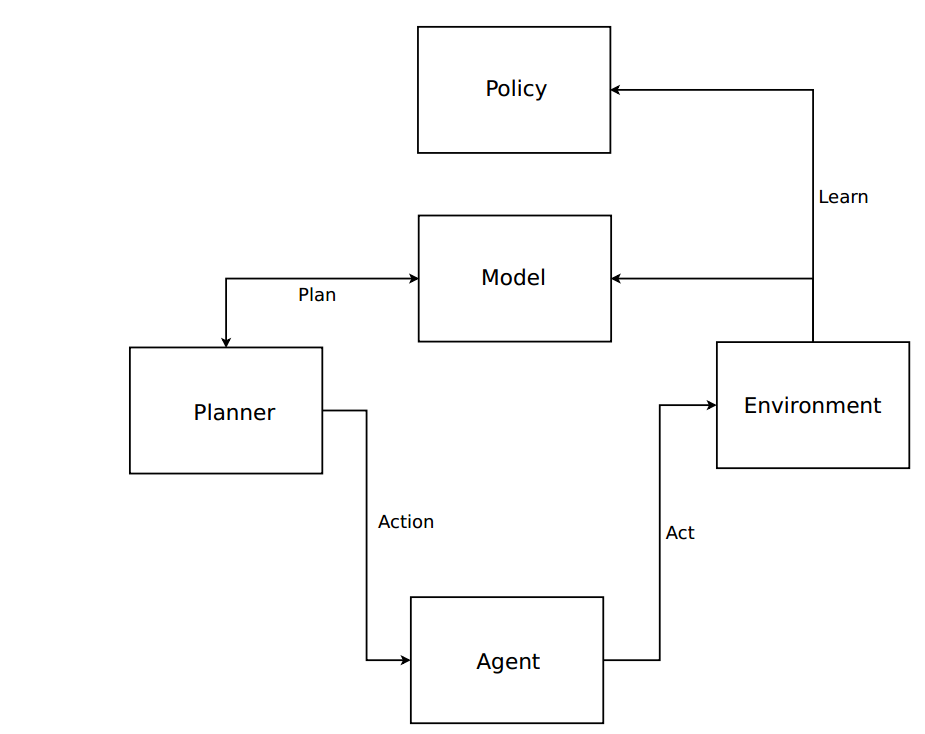
\includegraphics[max size={\textwidth}{\textheight}]{report/assets/planning_phase.png}
    \caption{Planning Phase}
    \label{fig:planning_phase}
\end{figure}

% Throughout the planing phase we maintain a tabular likelihood model which is used for model-learning, therefore we maintain a table $n$ which maps state-action-state triples to integers; for instance $(0, 1, 0) \rightarrow 3$ means that the transitions $(0, 1, 0)$ has been observed three times.
\subsubsection{Planning}
The planner constructs a temporary model, $M'$, which is identical to $M$. It then plans on $M'$ to produce a plan, $P$, from the current state $s$ to some goal, terminal, state $s_g$. The planner has access to the action space, $A$, as well as the additional Meta Actions. Whilst considering the Meta Actions, the planner may create additional temporary models, in order to evaluate the benefit of calling a particular Meta Action. If a Meta Action is chosen, then the temporary model $M'$ is updated, and planning continues. $P$ is maintained by the planner until $M$ is updated, when re-planning occurs. This ensures that unnecessary planning does not take place, saving on computational costs. However, this means that some mechanism needs to be in place for determining if the model has been altered since the last plan was generated; this can be a simple Boolean flag. $P$ is stored in a first-in, first-out (FIFO) data structure, such as a Queue. Thus, when the planner is invoked by the agent it simply removes and returns the top action.
\subsubsection{Acting}
At discrete time steps, $t$, the agent samples an action $a$ from the Planner, and executes it. At time $t+1$ it observes its new state $s'$ and the scalar reward signal.
\subsubsection{Learning}
The observation table is updated with the observed transition: $n(s, a, s') \leftarrow n(s, a, s')+1$, and if necessary the transition function, $T'$ of $M$ is updated by Equation \ref{eqn:tmlmupdate}. Furthermore, the reward function, $R'$, of $M$ is updated with the received reward, if necessary. $Q$ is updated according to the new state and reward received using Equation \ref{eqn:qlearningupdate}.
% We begin by updating the observation table $n$ with the observed transition. Then, we update the model, $M$ (if necessary). Furthermore, the $Q$-Function is updated according to the new state and reward received.
\subsection{The Model-Free Phase}
The model-free phase has two distinct steps: acting and learning, which can be seen in Figure \ref{fig:model_free_phase}. The goal of the model-free phase is to use pure model-free learning to bootstrap from the Q values learned during exploration, and get as close as possible to $Q^*$, so that $\pi^*$ can be derived.

\begin{figure}[h!]
    \centering
    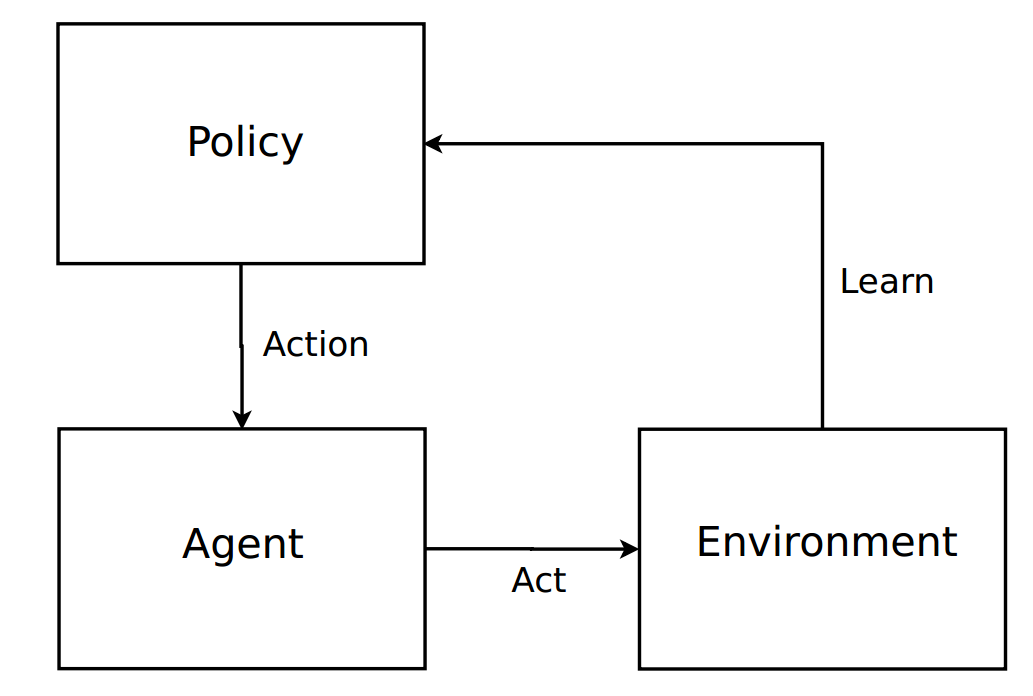
\includegraphics[max size={\textwidth}{\textheight}]{report/assets/model_free_phase.png}
    \caption{Model-Free Phase}
    \label{fig:model_free_phase}
\end{figure}

\subsubsection{Acting}
At discrete time steps, $t$, the agent greedily selections an action $a$ with respect to the $Q$, it selects the action according to the current policy, and executes it. At time $t+1$ it observes its new state $s'$ and the scalar reward signal.
\subsubsection{Learning}
$Q$ is updated according to the new state and reward received using Equation \ref{eqn:qlearningupdate}. Eventually, the updates will not result in changes to the policy, $\pi$, and therefore it will be continually followed until termination.
% \subsection{Planning}
% The choice of planner is largely irrelevant to the framework, we mostly consider heuristic search algorithms, through A*, and planning by dynamic programming, through Value Iteration. Value Iteration was chosen over Policy Iteration as it tends to be more efficient, and since we are performing VI many times; this is very beneficial. However, it is important for the planner to be able to quantitatively evaluate plans; planning by VI was a good option here, since it computed a Value Function as an intermediate step, and we could use that for evaluation.
% A temporary model is created. The planner then begins planning on this model, at each node (state), the planner considers both the actions and available Meta Actions - if a Meta Action is chosen, then that change is made to the temporary model and planning continues. The computed plan is then returned to the agent.
% \subsection{Execution}
% During the planning phase, the agent chooses actions by sampling a plan from the planner. During the model-free phase, the agent chooses actions from the learned policy. The agent then executes the action in the environment, observing its affects through its new state and the reward received.
% \subsection{Learning}
% There are two sections to the learning step: where the model is learned \citeppp{10.1145/122344.122377}, and  where the policy is learned. The model is learned, as a tabular maximum likelihood model. The policy is learned, by at each discrete time step  updating the maintained Q-values using Q-Learning.
% We acknowledge the fact that tabular maximum likelihood approach and tabular Q-function approaches do not scale well to large, continuous, state spaces, however the environments that we were interested in within this work had finite, discrete state spaces (or they could be discretised) which were not too large to suffer from the \textit{curse of dimensionality}. Moreover, these two choices allowed for simplifications to be made for ease of implementation. Q-Learning was chosen over SARSA, as it allows the optimal policy to be learned without actually following the optimal policy; this is key to the planning phase, where due to the hypotheses made, the policy being followed may not be optimal.
\section{An Illustrative Example}
Consider the gridworld in Figure {}. In the model the door is shown to be closed, however in the real environment the door is actually open. Since it would most benefit the agent if the door was open, a plan is hypothesised that imagines that the door is open. The agent tries this plan, realises the hypothesised changes to be correct and then updates its model.

\section{Implementations}
The description of the framework above led to various implementations. The underlying concept of allowing the planner to hypothesise changes to the model through Meta Actions is present throughout all of the implementations. However, the choice of planning algorithm differs. Each implementation will be presented and highlighted here. Since in general the implementations follow the high-level overview provided in Algorithm \ref{alg:framework_pc}, we will not provide pseudocodes for each individual implementation, but we will however note where implementations differ.
\subsection{RL-A* Meta}
This was the initial implementation of the framework, and therefore the planner used was a simple heuristic search algorithm, A*; due to this choice, the implementation was limited to deterministic domains. This decision was made, as this implementation aimed at discovering if and when Meta Actions were useful. A* in particular was chosen due to ease of implementation. Furthermore A* maintains an evaluation function, $f$, which provided a good means of evaluating hypothetical changes made through Meta Actions.
\begin{equation}
\label{eqn:astareval}
f : S \times A \times S \rightarrow \mathbb{R}
\end{equation}
For the cost function,  it was intuitive to use the inverted reward function, namely $-R'$, this ensured that states with very negative reward were assigned a high cost and vice versa, leading to the following definition:
\begin{equation}
\label{eqn:astarevalsas}
f(s,a,s') = -R(s, a, s') + h(s')
\end{equation}
The choice of heuristic, $h$, relies on domain specific knowledge, therefore we do not define it here. However,  it remains that the heuristic must be admissible. The transition function was treated as a graph, which A* search was then performed on.
\\The Meta Actions that were available to the planner allowed it to add/remove transitions, and increase/decrease rewards for state-action-state triples, reasonable meta actions were embedded in the model by-hand. To ensure feasibility of Meta Actions and ensure that they were not infinitely called, a table was maintained which kept track of which Meta Actions had been called on which state-action-triples - this was used to ensure that each Meta Action can only be called once on each state-action-state triple. 
\subsection{RL-A* Meta with short-term memory}
This implementation was an extension of RL-A* Meta, which aimed to scale to stochastic domains. The stochastic nature means that the evaluation function once again needed to be modified, as such:
\begin{equation}
\label{eqn:astarevalsast}
f(s, a, s') = (1-T(s, a, s'))(-R(s,a, s')) + h(s')
\end{equation}
Since transitions were not guaranteed, the cost was weighted using the probability of the transition not occurring.
\\ The Meta Actions that were available to the planner allowed it to increase/decrease transition probabilities and increase/decrease rewards for state-action-state triples. Reasonable meta actions were embedded in the model by-hand. To ensure feasibility of Meta Actions and ensure that they were not infinitely called, a table was maintained which kept track of which Meta Actions had been called on which state-action-triples in the previous $N$ episodes, this is the short term memory.
\subsection{RL-VI Meta}
This implementations aims to deal with varying domains. We opted for planning by dynamic programming, namely through Value Iteration. Value Iteration was chosen because it allowed for us to easily evaluate plans (policies) through the Value Function. We chose Value Iteration over Policy Iteration, as Value Iteration is generally faster, and we needed to perform it many times.
\\The Meta Actions that were available to the planner allowed it to add/remove transitions, and increase/decrease rewards for state-action-state tuples, reasonable meta actions were embedded in the model by-hand. Starting from an initial estimate of the optimal value function, $V$, the planner constructs a plan that is greedy with respect to $V$, however at each state, $s$, changes are hypothesised and verified to be beneficial by performing a few steps of value iteration to produce a temporary value function $V_h$. If $V_h(s) > V(s)$, then the change is accepted and the Meta Action is added to the plan.
To ensure feasibility of Meta Actions and ensure that they were not infinitely called, a table was maintained which kept track of Meta Actions called within the current episode.
\subsection{RL-VI Meta, with learned Meta Actions}
The overall implementation is the same as RL-VI Meta, except Meta Actions are learned and obtained through experience, rather than embedded by-hand in the model. A Meta Action is learned when a discrepancy is noticed between the model and the real environment; this change that was applied to the model through model-learning becomes an action that can be invoked later on.

% Adds references to the table of contents.
\addcontentsline{toc}{chapter}{References}
% All your bibtex entries should go in the file called "refs.bib".
\bibliography{refs}

% All appendices you have go in a file called "appendices.tex".
\begin{appendices}

%
% The first appendix must be "Self-appraisal".
%
\chapter{Self-appraisal}

<This appendix should contain everything covered by the 'self-appraisal' criterion in the mark scheme. Although there is no length limit for this section, 2---4 pages will normally be sufficient. The format of this section is not prescribed, but you may like to organise your discussion into the following sections and subsections.>

\section{Critical self-evaluation}

\section{Personal reflection and lessons learned}

\section{Legal, social, ethical and professional issues}

<Refer to each of these issues in turn. If one or more is not relevant to your project, you should still explain {\em why} you think it was not relevant.>

\subsection{Legal issues}

\subsection{Social issues}

\subsection{Ethical issues}

\subsection{Professional issues}


%
% Any other appendices you wish to use should come after "Self-appraisal". You can have as many appendices as you like.
%
\chapter{External Material}
<This appendix should provide a brief record of materials used in the solution that are not the student's own work. Such materials might be pieces of codes made available from a research group/company or from the internet, datasets prepared by external users or any preliminary materials/drafts/notes provided by a supervisor. It should be clear what was used as ready-made components and what was developed as part of the project. This appendix should be included even if no external materials were used, in which case a statement to that effect is all that is required.>




%
% Other appendices can be added here following the same pattern as above.
%



\end{appendices}


\end{document}

